%%%%%%%%%%%%%%%%%%%% author.tex %%%%%%%%%%%%%%%%%%%%%%%%%%%%%%%%%%%
%
% sample root file for your "contribution" to a contributed volume
%
% Use this file as a template for your own input.
%
%%%%%%%%%%%%%%%% Springer %%%%%%%%%%%%%%%%%%%%%%%%%%%%%%%%%%%%%%%%%


%% RECOMMENDED %%%%%%%%%%%%%%%%%%%%%%%%%%%%%%%%%%%%%%%%%%%%%%%%%%%
%\documentclass[graybox]{svmult}
%
%% choose options for [] as required from the list
%% in the Reference Guide
%
%\usepackage{mathptmx}       % selects Times Roman as basic font
%\usepackage{helvet}         % selects Helvetica as sans-serif font
%\usepackage{courier}        % selects Courier as typewriter font
%\usepackage{type1cm}        % activate if the above 3 fonts are
                             % not available on your system
%
%\usepackage{makeidx}         % allows index generation
%\usepackage{graphicx}        % standard LaTeX graphics tool
%                             % when including figure files
%\usepackage{multicol}        % used for the two-column index
%\usepackage[bottom]{footmisc}% places footnotes at page bottom
%
%% see the list of further useful packages
%% in the Reference Guide
%
%\makeindex             % used for the subject index
%                       % please use the style svind.ist with
%                       % your makeindex program
%
%%%%%%%%%%%%%%%%%%%%%%%%%%%%%%%%%%%%%%%%%%%%%%%%%%%%%%%%%%%%%%%%%%%%%%%%%%%%%%%%%%%%%%%%%%
%
%\begin{document}

\title{Contribution Title}
% Use \titlerunning{Short Title} for an abbreviated version of
% your contribution title if the original one is too long
\author{Name of First Author and Name of Second Author}
% Use \authorrunning{Short Title} for an abbreviated version of
% your contribution title if the original one is too long
\institute{Name of First Author \at Name, Address of Institute, \email{name@email.address}
\and Name of Second Author \at Name, Address of Institute \email{name@email.address}}
%
% Use the package "url.sty" to avoid
% problems with special characters
% used in your e-mail or web address
%
\maketitle

\abstract*{Each chapter should be preceded by an abstract (no more than 200 words) that summarizes the content. The abstract will appear \textit{online} at \url{www.SpringerLink.com} and be available with unrestricted access. This allows unregistered users to read the abstract as a teaser for the complete chapter.
Please use the 'starred' version of the \texttt{abstract} command for typesetting the text of the online abstracts (cf. source file of this chapter template \texttt{abstract}) and include them with the source files of your manuscript. Use the plain \texttt{abstract} command if the abstract is also to appear in the printed version of the book.}

\abstract{Each chapter should be preceded by an abstract (no more than 200 words) that summarizes the content. The abstract will appear \textit{online} at \url{www.SpringerLink.com} and be available with unrestricted access. This allows unregistered users to read the abstract as a teaser for the complete chapter.\newline\indent
Please use the 'starred' version of the \texttt{abstract} command for typesetting the text of the online abstracts (cf. source file of this chapter template \texttt{abstract}) and include them with the source files of your manuscript. Use the plain \texttt{abstract} command if the abstract is also to appear in the printed version of the book.}

\section{Section Heading}
\label{sec:1}
Use the template \emph{chapter.tex} together with the document class SVMono (monograph-type books) or SVMult (edited books) to style the various elements of your chapter content.

Instead of simply listing headings of different levels we recommend to let every heading be followed by at least a short passage of text. Further on please use the \LaTeX\ automatism for all your cross-references and citations. And please note that the first line of text that follows a heading is not indented, whereas the first lines of all subsequent paragraphs are.

\section{Section Heading}
\label{sec:2}
% Always give a unique label
% and use \ref{<label>} for cross-references
% and \cite{<label>} for bibliographic references
% use \sectionmark{}
% to alter or adjust the section heading in the running head
Instead of simply listing headings of different levels we recommend to let every heading be followed by at least a short passage of text. Further on please use the \LaTeX\ automatism for all your cross-references and citations.

Please note that the first line of text that follows a heading is not indented, whereas the first lines of all subsequent paragraphs are.

Use the standard \verb|equation| environment to typeset your equations, e.g.
%
\begin{equation}
a \times b = c\;,
\end{equation}
%
however, for multiline equations we recommend to use the \verb|eqnarray| environment\footnote{In physics texts please activate the class option \texttt{vecphys} to depict your vectors in \textbf{\itshape boldface-italic} type - as is customary for a wide range of physical subjects}.
\begin{eqnarray}
\left|\nabla U_{\alpha}^{\mu}(y)\right| &\le&\frac1{d-\alpha}\int
\left|\nabla\frac1{|\xi-y|^{d-\alpha}}\right|\,d\mu(\xi) =
\int \frac1{|\xi-y|^{d-\alpha+1}} \,d\mu(\xi)  \\
&=&(d-\alpha+1) \int\limits_{d(y)}^\infty
\frac{\mu(B(y,r))}{r^{d-\alpha+2}}\,dr \le (d-\alpha+1)
\int\limits_{d(y)}^\infty \frac{r^{d-\alpha}}{r^{d-\alpha+2}}\,dr
\label{eq:01}
\end{eqnarray}

\subsection{Subsection Heading}
\label{subsec:2}
Instead of simply listing headings of different levels we recommend to let every heading be followed by at least a short passage of text. Further on please use the \LaTeX\ automatism for all your cross-references\index{cross-references} and citations\index{citations} as has already been described in Sect.~\ref{sec:2}.

\begin{quotation}
Please do not use quotation marks when quoting texts! Simply use the \verb|quotation| environment -- it will automatically be rendered in line with the preferred layout.
\end{quotation}


\subsubsection{Subsubsection Heading}
Instead of simply listing headings of different levels we recommend to let every heading be followed by at least a short passage of text. Further on please use the \LaTeX\ automatism for all your cross-references and citations as has already been described in Sect.~\ref{subsec:2}, see also Fig.~\ref{fig:1}\footnote{If you copy text passages, figures, or tables from other works, you must obtain \textit{permission} from the copyright holder (usually the original publisher). Please enclose the signed permission with the manuscript. The sources\index{permission to print} must be acknowledged either in the captions, as footnotes or in a separate section of the book.}

Please note that the first line of text that follows a heading is not indented, whereas the first lines of all subsequent paragraphs are.

% For figures use
%
\begin{figure}[b]
\sidecaption
% Use the relevant command for your figure-insertion program
% to insert the figure file.
% For example, with the graphicx style use
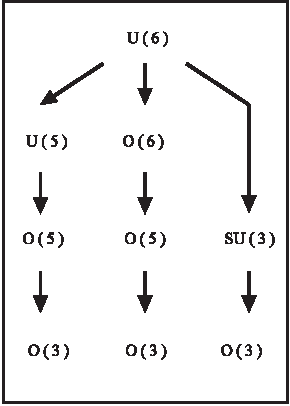
\includegraphics[scale=.65]{images/figure}
%
% If no graphics program available, insert a blank space i.e. use
%\picplace{5cm}{2cm} % Give the correct figure height and width in cm
%
\caption{If the width of the figure is less than 7.8 cm use the \texttt{sidecapion} command to flush the caption on the left side of the page. If the figure is positioned at the top of the page, align the sidecaption with the top of the figure -- to achieve this you simply need to use the optional argument \texttt{[t]} with the \texttt{sidecaption} command}
\label{fig:1}       % Give a unique label
\end{figure}


\paragraph{Paragraph Heading} %
Instead of simply listing headings of different levels we recommend to let every heading be followed by at least a short passage of text. Further on please use the \LaTeX\ automatism for all your cross-references and citations as has already been described in Sect.~\ref{sec:2}.

Please note that the first line of text that follows a heading is not indented, whereas the first lines of all subsequent paragraphs are.

For typesetting numbered lists we recommend to use the \verb|enumerate| environment -- it will automatically rendered in line with the preferred layout.

\begin{enumerate}
\item{Livelihood and survival mobility are oftentimes coutcomes of uneven socioeconomic development.}
\begin{enumerate}
\item{Livelihood and survival mobility are oftentimes coutcomes of uneven socioeconomic development.}
\item{Livelihood and survival mobility are oftentimes coutcomes of uneven socioeconomic development.}
\end{enumerate}
\item{Livelihood and survival mobility are oftentimes coutcomes of uneven socioeconomic development.}
\end{enumerate}


\subparagraph{Subparagraph Heading} In order to avoid simply listing headings of different levels we recommend to let every heading be followed by at least a short passage of text. Use the \LaTeX\ automatism for all your cross-references and citations as has already been described in Sect.~\ref{sec:2}, see also Fig.~\ref{fig:2}.

For unnumbered list we recommend to use the \verb|itemize| environment -- it will automatically be rendered in line with the preferred layout.

\begin{itemize}
\item{Livelihood and survival mobility are oftentimes coutcomes of uneven socioeconomic development, cf. Table~\ref{tab:1}.}
\begin{itemize}
\item{Livelihood and survival mobility are oftentimes coutcomes of uneven socioeconomic development.}
\item{Livelihood and survival mobility are oftentimes coutcomes of uneven socioeconomic development.}
\end{itemize}
\item{Livelihood and survival mobility are oftentimes coutcomes of uneven socioeconomic development.}
\end{itemize}

\begin{figure}[t]
\sidecaption[t]
% Use the relevant command for your figure-insertion program
% to insert the figure file.
% For example, with the option graphics use
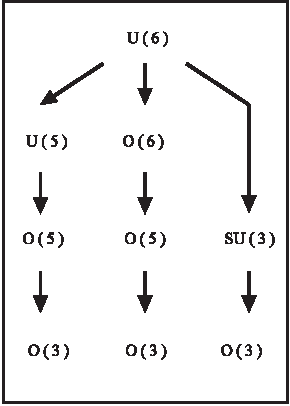
\includegraphics[scale=.65]{images/figure}
%
% If no graphics program available, insert a blank space i.e. use
%\picplace{5cm}{2cm} % Give the correct figure height and width in cm
%
%\caption{Please write your figure caption here}
\caption{If the width of the figure is less than 7.8 cm use the \texttt{sidecapion} command to flush the caption on the left side of the page. If the figure is positioned at the top of the page, align the sidecaption with the top of the figure -- to achieve this you simply need to use the optional argument \texttt{[t]} with the \texttt{sidecaption} command}
\label{fig:2}       % Give a unique label
\end{figure}

\runinhead{Run-in Heading Boldface Version} Use the \LaTeX\ automatism for all your cross-references and citations as has already been described in Sect.~\ref{sec:2}.

\subruninhead{Run-in Heading Boldface and Italic Version} Use the \LaTeX\ automatism for all your cross-refer\-ences and citations as has already been described in Sect.~\ref{sec:2}\index{paragraph}.

\subsubruninhead{Run-in Heading Displayed Version} Use the \LaTeX\ automatism for all your cross-refer\-ences and citations as has already been described in Sect.~\ref{sec:2}\index{paragraph}.
% Use the \index{} command to code your index words
%
% For tables use
%
\begin{table}[!t]
\caption{Please write your table caption here}
\label{tab:1}       % Give a unique label
%
% Follow this input for your own table layout
%
\begin{tabular}{p{2cm}p{2.4cm}p{2cm}p{4.9cm}}
\hline\noalign{\smallskip}
Classes & Subclass & Length & Action Mechanism  \\
\noalign{\smallskip}\svhline\noalign{\smallskip}
Translation & mRNA$^a$  & 22 (19--25) & Translation repression, mRNA cleavage\\
Translation & mRNA cleavage & 21 & mRNA cleavage\\
Translation & mRNA  & 21--22 & mRNA cleavage\\
Translation & mRNA  & 24--26 & Histone and DNA Modification\\
\noalign{\smallskip}\hline\noalign{\smallskip}
\end{tabular}
$^a$ Table foot note (with superscript)
\end{table}
%
\section{Section Heading}
\label{sec:3}
% Always give a unique label
% and use \ref{<label>} for cross-references
% and \cite{<label>} for bibliographic references
% use \sectionmark{}
% to alter or adjust the section heading in the running head
Instead of simply listing headings of different levels we recommend to let every heading be followed by at least a short passage of text. Further on please use the \LaTeX\ automatism for all your cross-references and citations as has already been described in Sect.~\ref{sec:2}.

Please note that the first line of text that follows a heading is not indented, whereas the first lines of all subsequent paragraphs are.

If you want to list definitions or the like we recommend to use the enhanced \verb|description| environment -- it will automatically rendered in line with the preferred layout.

\begin{description}[Type 1]
\item[Type 1]{That addresses central themes pertainng to migration, health, and disease. In Sect.~\ref{sec:1}, Wilson discusses the role of human migration in infectious disease distributions and patterns.}
\item[Type 2]{That addresses central themes pertainng to migration, health, and disease. In Sect.~\ref{subsec:2}, Wilson discusses the role of human migration in infectious disease distributions and patterns.}
\end{description}

\subsection{Subsection Heading} %
In order to avoid simply listing headings of different levels we recommend to let every heading be followed by at least a short passage of text. Use the \LaTeX\ automatism for all your cross-references and citations citations as has already been described in Sect.~\ref{sec:2}.

Please note that the first line of text that follows a heading is not indented, whereas the first lines of all subsequent paragraphs are.

\begin{svgraybox}
If you want to emphasize complete paragraphs of texts we recommend to use the newly defined class option \verb|graybox| and the newly defined environment \verb|svgraybox|. This will produce a 15 percent screened box 'behind' your text.

If you want to emphasize complete paragraphs of texts we recommend to use the newly defined class option and environment \verb|svgraybox|. This will produce a 15 percent screened box 'behind' your text.
\end{svgraybox}


\subsubsection{Subsubsection Heading}
Instead of simply listing headings of different levels we recommend to let every heading be followed by at least a short passage of text. Further on please use the \LaTeX\ automatism for all your cross-references and citations as has already been described in Sect.~\ref{sec:2}.

Please note that the first line of text that follows a heading is not indented, whereas the first lines of all subsequent paragraphs are.

\begin{theorem}
Theorem text goes here.
\end{theorem}
%
% or
%
\begin{definition}
Definition text goes here.
\end{definition}

\begin{proof}
%\smartqed
Proof text goes here.
%\qed
\end{proof}

\paragraph{Paragraph Heading} %
Instead of simply listing headings of different levels we recommend to let every heading be followed by at least a short passage of text. Further on please use the \LaTeX\ automatism for all your cross-references and citations as has already been described in Sect.~\ref{sec:2}.

Note that the first line of text that follows a heading is not indented, whereas the first lines of all subsequent paragraphs are.
%
% For built-in environments use
%
\begin{theorem}
Theorem text goes here.
\end{theorem}
%
\begin{definition}
Definition text goes here.
\end{definition}
%
\begin{proof}
%\smartqed
Proof text goes here.
%\qed
\end{proof}
%
\begin{trailer}{Trailer Head}
If you want to emphasize complete paragraphs of texts in an \verb|Trailer Head| we recommend to
use  \begin{verbatim}\begin{trailer}{Trailer Head}
...
\end{trailer}\end{verbatim}
\end{trailer}
%
\begin{question}{Questions}
If you want to emphasize complete paragraphs of texts in an \verb|Questions| we recommend to
use  \begin{verbatim}\begin{question}{Questions}
...
\end{question}\end{verbatim}
\end{question}
\eject%
\begin{important}{Important}
If you want to emphasize complete paragraphs of texts in an \verb|Important| we recommend to
use  \begin{verbatim}\begin{important}{Important}
...
\end{important}\end{verbatim}
\end{important}
%
\begin{warning}{Attention}
If you want to emphasize complete paragraphs of texts in an \verb|Attention| we recommend to
use  \begin{verbatim}\begin{warning}{Attention}
...
\end{warning}\end{verbatim}
\end{warning}

\begin{programcode}{Program Code}
If you want to emphasize complete paragraphs of texts in an \verb|Program Code| we recommend to
use

\verb|\begin{programcode}{Program Code}|

\verb|\begin{verbatim}...\end{verbatim}|

\verb|\end{programcode}|

\end{programcode}
%
\begin{tips}{Tips}
If you want to emphasize complete paragraphs of texts in an \verb|Tips| we recommend to
use  \begin{verbatim}\begin{tips}{Tips}
...
\end{tips}\end{verbatim}
\end{tips}
\eject%
\begin{overview}{Overview}
If you want to emphasize complete paragraphs of texts in an \verb|Overview| we recommend to
use  \begin{verbatim}\begin{overview}{Overview}
...
\end{overview}\end{verbatim}
\end{overview}
\begin{backgroundinformation}{Background Information}
If you want to emphasize complete paragraphs of texts in an \verb|Background|
\verb|Information| we recommend to
use

\verb|\begin{backgroundinformation}{Background Information}|

\verb|...|

\verb|\end{backgroundinformation}|
\end{backgroundinformation}
\begin{legaltext}{Legal Text}
If you want to emphasize complete paragraphs of texts in an \verb|Legal Text| we recommend to
use  \begin{verbatim}\begin{legaltext}{Legal Text}
...
\end{legaltext}\end{verbatim}
\end{legaltext}
%
\begin{acknowledgement}
If you want to include acknowledgments of assistance and the like at the end of an individual chapter please use the \verb|acknowledgement| environment -- it will automatically be rendered in line with the preferred layout.
\end{acknowledgement}
%
\section*{Appendix}
%\addcontentsline{toc}{section}{Appendix}
%
%
When placed at the end of a chapter or contribution (as opposed to at the end of the book), the numbering of tables, figures, and equations in the appendix section continues on from that in the main text. Hence please \textit{do not} use the \verb|appendix| command when writing an appendix at the end of your chapter or contribution. If there is only one the appendix is designated ``Appendix'', or ``Appendix 1'', or ``Appendix 2'', etc. if there is more than one.

\begin{equation}
a \times b = c
\end{equation}

\part{References}\label{part:refs}

\printbibheading

% \bibbysegment[heading=subbibliography,nottype=misc]
\printbibliography[segment=1,nottype=software,title={Earthquake - Ground Shaking}]
\printbibliography[segment=2,nottype=software,title={Earthquake - Surface Fault Rupture}]
\printbibliography[segment=3,nottype=software,title={Earthquake - Soil Liquefaction}]
\printbibliography[segment=4,nottype=software,title={Earthquake - Slope Stability and Landslides}]
\printbibliography[segment=5,nottype=software,title={Tropical Cyclone - Wind}]
\printbibliography[segment=6,nottype=software,title={Tropical Cyclone - Storm Surge}]
\printbibliography[segment=7,nottype=software,title={Tsunami - Inundation}]
\printbibliography[segment=8,nottype=software,title={Structural Systems}]
\printbibliography[segment=9,nottype=software,title={Geotechnical Systems}]
\printbibliography[segment=10,nottype=software,title={Computational Cluid Dynamics - Wind}]
\printbibliography[segment=11,nottype=software,title={Computational Cluid Dynamics - Water}]
\printbibliography[segment=12,nottype=software,title={Buildings}]
\printbibliography[segment=13,nottype=software,title={Transportation Networks}]
\printbibliography[segment=14,nottype=software,title={Water, Sewer, and Gas Pipelines}]
\printbibliography[segment=15,nottype=software,title={Electrical Transmission Substations and Lines}]
\printbibliography[segment=16,nottype=software,title={Communities}]
\printbibliography[segment=17,nottype=software,title={Infrastructure Systems}]
\printbibliography[segment=18,nottype=software,title={Housing}]
\printbibliography[segment=19,nottype=software,title={Business}]
\printbibliography[segment=20,nottype=software,title={Uncertainty Quantification}]
\printbibliography[segment=21,nottype=software,title={Artificial Intelligence and Machine Learning}]
%---------------------------------------------
\defbibenvironment{bibliography}
{\list
{\printfield[labelnumberwidth]{labelnumber}}
{\setlength{\labelwidth}{\labelnumberwidth}%
\setlength{\leftmargin}{\labelwidth}%
\setlength{\labelsep}{\biblabelsep}%
\addtolength{\labelsep}{1em}
\addtolength{\leftmargin}{\labelsep}%
\setlength{\itemsep}{\bibitemsep}%
\setlength{\parsep}{\bibparsep}}%
\renewcommand*{\makelabel}[1]{\hss##1}}
{\endlist}
{\item}
\DeclareFieldFormat{labelnumberwidth}{\mkbibbrackets{#1}\hspace{-1.1em}}

\section*{Software}

% \printbibliography[type=software,resetnumbers,title=Programs]
\printbibliography[segment=1,resetnumbers,type=software,title={Earthquake - Ground Shaking}]
\printbibliography[segment=2,resetnumbers,type=software,title={Earthquake - Surface Fault Rupture}]
\printbibliography[segment=3,resetnumbers,type=software,title={Earthquake - Soil Liquefaction}]
\printbibliography[segment=4,type=software,title={Earthquake - Slope Stability and Landslides}]
\printbibliography[segment=5,type=software,title={Tropical Cyclone - Wind}]
\printbibliography[segment=6,type=software,title={Tropical Cyclone - Storm Surge}]
\printbibliography[segment=7,type=software,title={Tsunami - Inundation}]
\printbibliography[segment=8,type=software,title={Structural Systems}]
\printbibliography[segment=9,type=software,title={Geotechnical Systems}]
\printbibliography[segment=10,type=software,title={Computational Cluid Dynamics - Wind}]
\printbibliography[segment=11,type=software,title={Computational Cluid Dynamics - Water}]
\printbibliography[segment=12,type=software,title={Buildings}]
\printbibliography[segment=13,type=software,title={Transportation Networks}]
\printbibliography[segment=14,type=software,title={Water, Sewer, and Gas Pipelines}]
\printbibliography[segment=15,type=software,title={Electrical Transmission Substations and Lines}]
\printbibliography[segment=16,type=software,title={Communities}]
\printbibliography[segment=17,type=software,title={Infrastructure Systems}]
\printbibliography[segment=18,type=software,title={Housing}]
\printbibliography[segment=19,type=software,title={Business}]
\printbibliography[segment=20,type=software,title={Uncertainty Quantification}]
\printbibliography[segment=21,type=software,title={Artificial Intelligence and Machine Learning}]
%---------------------------------------------


%%%%%%%%%%%%%%%%%%%%%%%%%%%%%%%%%%%%%%%%%%%%%%%%%%%%%%%%%%%%%%%%%%%%%%



%\end{document}
